\chapter{Experiment with Getafix}
	\label{CH_03}

\marginpar{(why and what other property are there)}
We want to use model-checking tools to see if we can reduce the time requirement of algorithm \ref{code:doubleLoop}. Specifically, we choose the reachability property and append algorithm \ref{code:reachLine} to the end of algorithm \ref{code:doubleLoop}. The statement within the if statement has a label. Although the exact statement following that label is irrelevant, reaching this line means $OCounter$ satisfies the constrains in the condition block.

\marginpar{correct citations of web page}
We experiment on several model-checking tools, including Interproc from \cite{_interproc_2011}, Berkeley Lazy Abstraction Software Verification Tool (Blast) from \cite{_mtc_2008} and Getafix from \cite{la_torre_analyzing_2009}. We can not get correct reachability results from Interproc and Blast, so we shift our focus onto Getafix.

\renewcommand{\algorithmiccomment}[1]{// #1}
\begin{algorithm}
\begin{algorithmic}

\IF{value of $OCounter$ meets certain constrains}
\STATE reach: $OCounter$
\COMMENT{a label followed by a statement}
\ENDIF

\end{algorithmic}

\caption[Single loop]{Determine if $OCounter$ meets certain constrains.}
\label{code:reachLine}
\end{algorithm}

\section{Getafix}
\marginpar{Mostly copied from getafix website. Need rewrite}
Getafix is a symbolic model checker for Boolean programs implemented in \cite{la_torre_analyzing_2009}. Getafix only supports reachability check. It translates sequential and concurrent Boolean programs into Boolean formulae and uses the model-checker Mucke to solve the reachability problem symbolically using Boolean Decision Diagrams \cite{_getafix_2009}. 

\begin{figure}
\centering
\caption{Converter, Getafix and Mucke complet workflow}
\label{fig:workFlow}
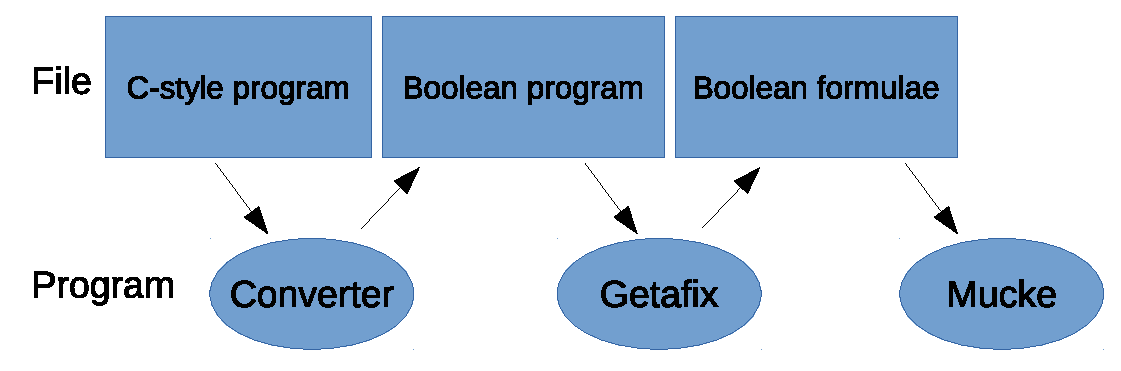
\includegraphics[scale=0.8]{Figures/workFlow}
\end{figure}

\section{The converter}
Input for Getafix are boolean programs, meaning it only supports binary variables which can be either 0 or 1. We represent our problem in c-style code, thus we need to translate it into boolean form. We implemented a converter to automate this process, and figure \ref{fig:workFlow} shows the complete workflow including the converter. The converter has three components, a parser, a built-in function generator and a piece of script which calls the first two components and assemble the output file. The converter has these properties:
\begin{enumerate}
\item The input to the converter is a c-style code file and a positive integer which represent the bit length. The converter supports 32 bits and less. Also note that the converter represents a number with bit length of $bitLength$ using $bitLength + 1$ bits. We do this so that writing a loop which iterate from $0$ to $1<<bitLength - 1$ is easier.
\item The output of the converter is a boolean program which follows the syntax of Getafix input file.
\item In the language that we defined for the input file, we support only one variable type: non-negative decimal integer. Again we support the length up to 32 bits.
\item Our converter does not support function definitions. The input file has two parts, variable declarations block and statements block. The parser will print these blocks into the main function of the output boolean program. Also we require all variable declarations to appear before statements in the input code. Getafix input syntax has this requirement, and we decide to keep it in our converter.
\item We implement support for the following symbolic operators in the language: plus +, minus -, and \&, or $|$, xor \textasciicircum , greater than \textgreater, equal ==, less than \textless, not equal !=, greater than or equal \textgreater=, less than or equal \textless=, left shift \textless\textless and right shift \textgreater\textgreater.
\item We implement support for three control statements: if...else, while loop, goto and statements with labels. We currently do not support for loop, do...while loop, switch statements, break and continue, but these statements can be easily expressed using the supported ones.
\end{enumerate}

Input to the parser is a c-style code file and a desired bit length. Output of the parser is its corresponding boolean program which follows the syntax of Getafix input file. First we define the syntax of the input code and second we create the parser using flex and bison. The parser scans the input code and builds a syntax tree. Then the parser prints the syntax tree as a boolean program. The parser has three points worth noting:

\begin{table}[h]
\caption{Examples of input and output of the parser, with bit length of 4}
\label{tbl:parser-example}
\begin{tabular}{|l|l|}
\hline
Input& Output  \\ \hline
var SMax = 16;     & \begin{tabular}[c]{@{}l@{}}decl SMax4,SMax3,SMax2,SMax1,SMax0;\\ Smax4, SMax3, SMax2, SMax1, SMax1 := 1,0,0,0,0;\end{tabular} \\ \hline
STemp = STemp - 5; & \begin{tabular}[c]{@{}l@{}}STemp4,STemp3,STemp2,STemp1,STemp0 := \\ minus(STemp4,STemp3,STemp2,STemp1,STemp0,0,0,1,0,1); \end{tabular} \\ \hline
\end{tabular}
\end{table}

\begin{enumerate}
\item When printing the output code, the parser ``stretches'' each variable and literal into its binary form. Assume the desired bit length is $bitLength$. We split each variable into $bitLength$ variables by copying the name of the variable $bitLength$ times and append a counter value to each one. Also we convert a literal to its corresponding binary value and prepend it with zeros to reach the desired length. Table \ref{tbl:parser-example} contains an example of how the parser deals with a variable declaration.
\item In a boolean program, all operators operate on bit level, so we need to implement higher-level operators like plus, minus, greater than and left shift using operators that Getafix supports. In the parser, we print these high-level operators as function calls in the output boolean program, and the built-in function generator generates the body of the function. Table \ref{tbl:parser-example} contains an example of how the parser deals with a high-level operator.
\item In the boolean code syntax which Getafix defines, function call plus the semicolon is defined as a statement, and another rule allows the code to assign a function call to an identifier, but function call itself is not an expression. This means that a function call can not work as an expression as in many other languages, and it leads to two problems: First, the decider expression in if...else and while statements can not contain function calls. Second, parameters of a function call or operands to an operator can not be a function call. We automated a solution in the parser to the first problem, which assigns the decider expression to a temporary variable and use that variable as the decider, so we can use the c-style if...else and while in the input code. For the second problem, a possible solution would be to manage a set of internal temporary variables and assign each function call to a variable, but we did not implement it.
\end{enumerate}

Input to the built-in function generator is a desired bit length. Output is a set of high-level operators like plus and left shift implemented as functions. We do not track the necessary functions in the parser, as experiments with Getafix indicate that the uncalled functions affect little on the execution time. Listing \ref{lst:isGT} shows a sample function by the generator.

\lstset{language=C}  
\begin{lstlisting}[caption={Greater than operator as a function in boolean program with bit length of 2.},label=lst:isGT]
bool isGT(left2,left1,left0,right2,right1,right0)
begin
if (left2 != right2) then
	if (left2 = 1) then
		return 1;
	fi
else 
	if (left1 != right1) then
		if (left1 = 1) then
			return 1;
		fi
	else 
		if (left0 != right0) then
			if (left0 = 1) then
				return 1;
			fi
		fi
	fi
fi
return 0;
end
\end{lstlisting}

Input to the third component, a piece of script, is a c-style code file and a desired bit length. Output of the script is a boolean program ready for Getafix to process. The script first passes the bit length to the built-in function generator and redirect its output to the output file. Then the script passes both the input to the parser and append its output to the output file. At this point the output is complete.

\section{Tests and results}
Before we have the converter, we coded a test case manually and Getafix gave us the correct answer. Now with the converter we can run more complicated tests and see if Getafix is a good solution to the problem of calculating information leakage. We decide to run the ten test cases from paper \cite{meng_calculating_2011}. In each test, $O$ represents the output of its test, and $S$ is the input.
 
\subsection{Sanity check}
Listing \ref{lst:sanityCheck} shows the code we use. In this test, $O$ remains constant unless $S$ is within a certain range. The program has 16 different outputs, ranging from $4$ to $19$.

\lstset{language=C}  
\begin{lstlisting}[caption={Sanity check test program.},label=lst:sanityCheck]
var base = 4;
if(S < 16){O = base+ S;}
else{O = base;}
\end{lstlisting}
